\documentclass[12pt]{article}
\usepackage[margin=0.1in]{geometry}
\usepackage{arev}
\usepackage{pgfplots}
\usetikzlibrary{calc}
\pgfplotsset{compat=newest}

\begin{document}
\begin{figure}[h]
    \centering
    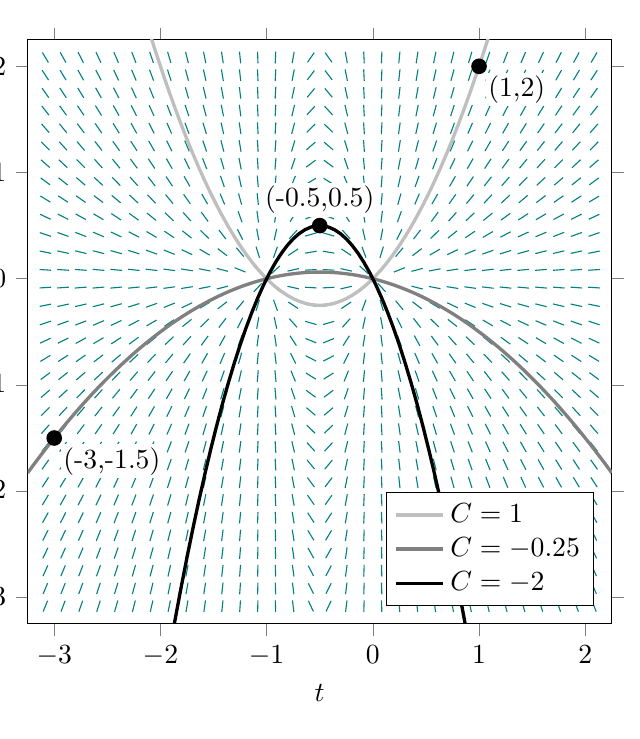
\begin{tikzpicture}[
            trim axis left, trim axis right, % options to centre correctly
            declare function={
            dydx(\x,\y) = (2*\x+1)*\y / ((\x)^2+\x); % differential equation
            solution(\x,\c) = \c*(\x^2 + \x); % general solution including constant of integration
            }
        ]

        % axes settings
        \def\width{9cm} \def\height{9cm}
        \def\xmin{-3.25} \def\xmax{2.25}
        \def\ymin{-3.25} \def\ymax{2.25}
        \def\xticks{\xmin+0.25,...,\xmax-0.25}
        \def\yticks{\xticks}

        \begin{axis}[
            view = {0}{90}, % set camera to point towards x-y plane
            domain=\xmin:\xmax, xmin=\xmin, xmax=\xmax, ymin=\ymin, ymax=\ymax, xtick=\xticks, ytick=\yticks,
            xlabel=$t$, ylabel=$w$,
            tick align=outside,
            width=\width, height=\height,
            legend pos=south east, legend cell align={left}, axis equal image ]

        % Plot slope field by iterating through each point in a grid
        % \foreach doesn't expand macros in and axis environment, so use \pgfplotsinvokeforeach
        % but \pgfplotsinvokeforeach can't be nested, so need to use mod() and int() for columns and rows
        % See https://tex.stackexchange.com/questions/170664 for details
        \def\numSlopes{32}
        \pgfmathsetmacro{\scale}{(\xmax-\xmin)/50}
        \pgfmathsetmacro{\hx}{(\xmax-\xmin)/(\numSlopes+1)} % +2 to account for the slopes at the domain edge that aren't drawn
        \pgfmathsetmacro{\hy}{(\ymax-\ymin)/(\numSlopes+1)}
        \pgfmathsetmacro{\totalSlopes}{\numSlopes^2-1}
        \pgfplotsinvokeforeach{0,...,\totalSlopes} {
            \pgfmathparse{mod(#1, \numSlopes))}\edef\i{\pgfmathresult}
            \pgfmathparse{int(#1 / \numSlopes)}\edef\j{\pgfmathresult}
            \pgfmathparse{dydx({\hx+\xmin+\i*\hx}, {\hy+\ymin+\j*\hy})}\edef\slope{\pgfmathresult}
            \pgfmathparse{\scale/sqrt((\slope)^2+1)}\edef\dx{\pgfmathresult}
            \pgfmathparse{\slope*\dx}\edef\dy{\pgfmathresult}
            \edef\tmp{\noexpand\draw[teal] ({\hx+\xmin+\i*\hx-\dx/2},{\hy+\ymin+\j*\hy-\slope*\dx/2})--({\hx+\xmin+\i*\hx+\dx/2},{\hy+\ymin+\j*\hy+\slope*\dx/2});}\tmp
        }

        % #1: coordinates of node, #2: relative position of node label (can also be angle)
        \newcommand\labelledPoint[2]{\node[circle, fill, inner sep=2pt, label={[fill=white,distance=1pt,inner sep=1pt]#2:{(#1)}}] at (#1){}}

        % plot initial points and corresponding solution curves
        \addplot[very thick, black!25, samples=100] {solution(x, 1)};
        \labelledPoint{1,2}{below right};

        \addplot[very thick, black!50, samples=100] {solution(x, -0.25)};
        \labelledPoint{-3,-1.5}{below right};

        \addplot[very thick, black!100, samples=100] {solution(x, -2)};
        \labelledPoint{-0.5,0.5}{above};

        % add legend, ignoring quiver plot
        \legend{$C=1$, $C=-0.25$, $C=-2$}
        \end{axis}

    \end{tikzpicture}
\end{figure}
\end{document}
